\documentclass[t, pdftex, aspectratio=169]{beamer}  % for 16:9 slides
\usetheme{CambridgeUS}
\usecolortheme{crane}

\usepackage{graphicx}
\graphicspath{{./figs/}}
\DeclareGraphicsExtensions{.pdf,.jpeg,.png, .jpg, .PNG}

\usepackage{tikz}
\usetikzlibrary{arrows}
\usetikzlibrary {arrows.meta}
\usetikzlibrary{intersections}
\usetikzlibrary{calc, quotes}
\usetikzlibrary{external}
\usetikzlibrary{positioning}
\usetikzlibrary{shapes.geometric, shapes.misc}
\usetikzlibrary{tikzmark}
\usetikzlibrary{decorations.pathreplacing}

\title{Towards a Better Verification Function}
\author{Lixun Zhang}
\date{\today}


\begin{document}
\frame{\maketitle}

\begin{frame}{Outline}
    \tableofcontents
\end{frame}

\section{Motivation}

\begin{frame}
  \frametitle{Verification Method in MLIR}
  \textbf{Verification}: compare outputs from GPU kernel (kern) and validation function (val)
  \vskip+1em
  \uncover<2->
  {Current verification method used by MLIR
    \begin{equation}
      \text{maxRelDiff}_\text{old} = \max\limits_i(\frac{|\text{val}_i - \text{kern}_i|}{|\text{val}_i|}), \; |\text{val}_i|>1\times10^{-3}\nonumber
    \end{equation}
    \vskip-1em
    \begin{itemize}
    \item Element wise metric
    \item Relative error between two values
    \item Ignore the error if the denominator is too small ($< 1\times10^{-3}$)
    \item Pass if the maximum relative difference among all elements is smaller than a tolerance $\delta_{rel}$
    \end{itemize}}

  \uncover<3->
  {Problem: $\delta_{rel} = 15\%$ for fp16 tests with random inputs ([-1, 1])
    \begin{itemize}
    \item MLIR\#408, PR\#694, PR\#696
    \item \alert{$\delta_{rel}$ is too large to distinguish bugs from numerical errors}
    \item For other data types, $\delta_{rel}=1\times10^{-6}$ 
    \end{itemize}}
\end{frame}

\begin{frame}
  \frametitle{Verification Method in  MIOpen}

  Current verification method used by MIOpen: RMS
  \begin{columns}
    
    \column{0.6\linewidth}
    \vskip-1em
    \begin{itemize}
    \item global metric
    \item Pass if RMS is smaller than a tolerance $\delta_{RMS}$
    \item Adjust $\delta_{RMS}$ for different directions, algorithms, data types, and issues
    \end{itemize}

    \column{0.4\linewidth}
    \vskip-3em
    \begin{equation}
      \frac{\sqrt{\sum\limits_{i=1}^N(a_i-b_i)^2}}{\sqrt{N}\cdot\max(\max(|a_i|), \max(|b_i|))}\nonumber
    \end{equation}
  \end{columns}
  
  \vskip+.5em
  {\centering 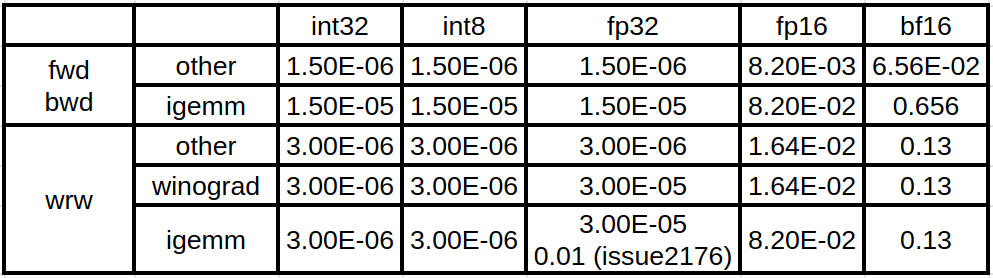
\includegraphics[width=3.5in]{miopen_rms}}

  Pro/con of RMS as a measure of difference
  \begin{itemize}
  \item Insensitive to element wise differences
  \end{itemize}
\end{frame}

\begin{frame}
  \frametitle{Element wise vs. RMS}
  \begin{columns}

    \column{0.5\linewidth}

    Element wise metric
    \begin{itemize}
    \item compare each element
    \item pick the maximum difference
    \item sensitive to large differences for individual elements
    \item false alarm caused by numerical errors
    \end{itemize}
    
    \column{0.5\linewidth}

    Aggregated global metric
    \begin{itemize}
    \item compare each element
    \item aggregate differences from all elements
    \item insensitive to large differences for individual elements
    \item false negative and miss a real bug
    \end{itemize}
  \end{columns}

  \vskip+1em
  \uncover<2->
  {We need a better verification function that can \alert{detect bugs and ignore numerical errors}
    \begin{itemize}
    \item which metric to use? Element wise or RMS?
    \item how to choose $\delta$?
    \item how to deal with special tests?
    \end{itemize}}
\end{frame}



\section{Experiment}

\subsection{Methodology and Setup}

\begin{frame}
  \frametitle{Other Element Wise Metrics}

  \begin{itemize}
  \item Absolute difference $\text{maxAbsDiff} = \max\limits_i(|\text{val}_i - \text{kern}_i|)$
    % \begin{equation}
    %   \text{maxAbsDiff} = \max\limits_i(|\text{val}_i - \text{kern}_i|)\nonumber
    % \end{equation}
  \item Relative difference (ignore zero denominators)
    \begin{equation}
      \text{maxRelDiff} = \max\limits_i(\frac{|\text{val}_i - \text{kern}_i|}{|\text{val}_i|}), \; |\text{val}_i|>0\nonumber
    \end{equation}
  \item Relative difference w.r.t $\epsilon$
    \begin{equation}
      \text{maxEpsilonDiff} = \max\limits_i(\frac{|\text{val}_i - \text{kern}_i|}{\epsilon_{|\text{val}_i|}})\nonumber
    \end{equation}
    where $\epsilon_{|\text{val}_i|}$ is the precision of fp16 numbers around $\text{val}_i$.
  \end{itemize}
  
\end{frame}


\begin{frame}
  \frametitle{Experiment Setup}

  \vskip-1em
  \begin{columns}
    \column{0.6\linewidth}

    Sources of configs: auto\_e2e/ e2e\_for\_pr/ misc\_e2e/
    % \vskip+.5em
    {\centering 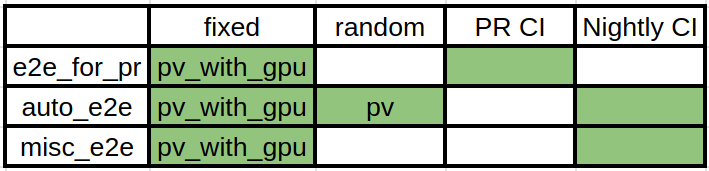
\includegraphics[width=3in]{tests}}

    \column{0.4\linewidth}

    \uncover<3->
    {Hardware
      \begin{itemize}
      \item MI100 gfx908 ixt-rack-112
      \item MI200 gfx90a lockhart5
      \end{itemize}}
  \end{columns}
  
  \vskip+.5em
  \uncover<2->
  {Settings of the test
    \begin{itemize}
    \item \texttt{-rand} 1: Generate random numbers as inputs
    \item \texttt{-rand\_min} and \texttt{-rand\_max}: choose the range of the random numbers
      \begin{itemize}
      \item r0 [-1, 1],  r1 [-10, 10], r4 [1, 5], r5 [5, 10]
      \end{itemize}
    \item \texttt{-pv} and \texttt{-pv\_with\_gpu}: choose the validation method
    \item \texttt{-x2}: enable xdlops
    \end{itemize}}

  \uncover<4->
  {Methodology: \alert{Effects of different settings to the error w.r.t all metrics}}
\end{frame}


\subsection{Results and Observations}

\begin{frame}
  \frametitle{Flush-denorms-to-zero}

  \begin{tikzpicture}
    \coordinate (tab TL) at (0, 1);
    
    \draw [fill=cyan] (tab TL) circle (2pt);

    \node [below right, inner sep=0] at (tab TL){
      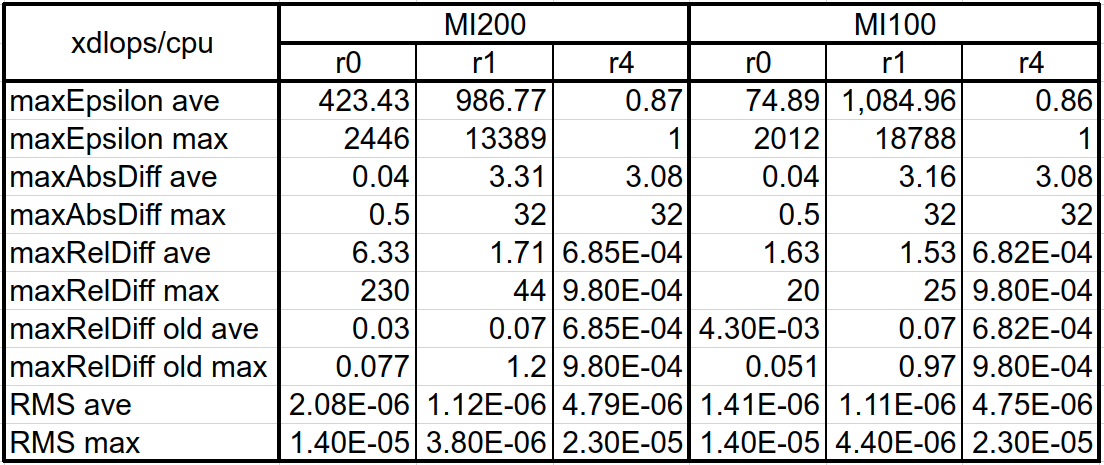
\includegraphics[width=3.8in]{flush-denorm-to-zero}}; 

    %% table name
    \node [below right, align=left, scale=.9] at ($(tab TL)+(9.7, 0)$)
    {\texttt{mfma} instructions flush subnormal\\
      numbers ($< 2^{-14}$) to zero on MI200\\
      r0 [-1, 1]\\r1 [-10, 10]\\r4 [1, 5]};
    %% Exceptions
    \uncover<2>
    { \draw [brown, thick] ($(tab TL)+(0.03, -3.4)$) rectangle ++(9.6, -.66);
      \draw [brown, thick] ($(tab TL)+(0.03, -2.05)$) rectangle ++(4.8, -.66);}
    \uncover<3>
    { \draw [red, thick] ($(tab TL)+(2.5, -.4)$) rectangle ++(1.1, -3.6);
      \draw [red, thick] ($(tab TL)+(6.1, -.4)$) rectangle ++(1.1, -3.6);}
    \uncover<4>
    { \draw [blue, thick] ($(tab TL)+(4.9, -.4)$) rectangle ++(1.1, -3.6);
      \draw [blue, thick] ($(tab TL)+(8.5, -.4)$) rectangle ++(1.1, -3.6);}
    
    
    % \draw [blue, thick] ($(tab TL)+(5.1, -2.1)$) rectangle ++(2.45, -.6);
  \end{tikzpicture}

  \begin{itemize}
  \item flush-denorms-to-zero behavior leads to
    \begin{itemize}
      \uncover<2->
      {\item $E_{r1} > E_{r0}$ on both MI200 and MI100 (except for maxRelDiff and RMS)}
      \uncover<3->
      {\item $E_{MI200}>E_{MI100}$ with r0}
      \uncover<4->
      {\item  $E_{MI200} \approx E_{MI100}$ with r4}
    \end{itemize}
  \end{itemize}
 
\end{frame}

\begin{frame}
  \frametitle{Underflow and Overflow}

  \begin{columns}
    \column{0.4\linewidth}

    \begin{tikzpicture}[overlay, remember picture]
      \coordinate (tab TL) at (0, 1);
      
      \draw [fill=cyan] (tab TL) circle (2pt);

      \node [below right, inner sep=0] at (tab TL){
        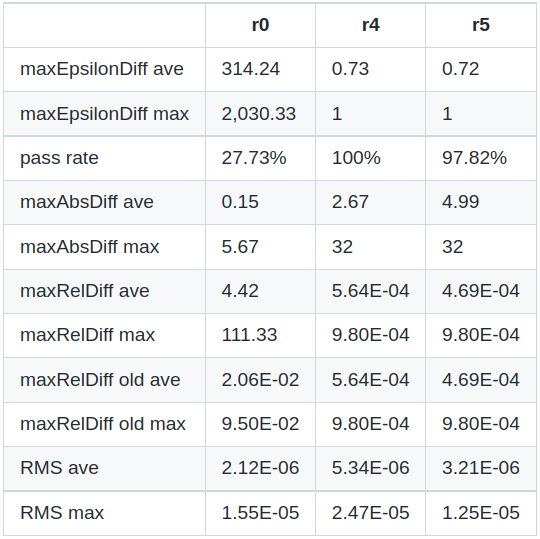
\includegraphics[width=2.5in]{Underflow_overflow}}; 

      %% table name
      \node [below right, align=left] at ($(tab TL)+(0, -4.5)$)
      { r0 [-1, 1] vs. r4 [1, 5]/r5 [5, 10]};
      \uncover<2->
      { \node [below right, align=left] at ($(tab TL)+(0, -5)$)
        { A test passes if $\text{maxEpsilonDiff} \le 1$};}
      %% Exceptions
      \uncover<1>
      { \draw [brown, thick] ($(tab TL)+(0.03, -1.75)$) rectangle ++(6.3, -.6);
        \draw [brown, thick] ($(tab TL)+(0.03, -3.77)$) rectangle ++(6.3, -.66);}
      \uncover<2>
      { \draw [blue, thick] ($(tab TL)+(0.03, -1.4)$) rectangle ++(6.3, -.3);}
      \uncover<3->
      { \draw [red, thick] ($(tab TL)+(3.8, -1.1)$) rectangle ++(2.5, -.6);}
    \end{tikzpicture}
    \column{0.55\linewidth}

    \begin{itemize}
    \item Errors with r0 is larger than that of r4/r5\\
      $\Leftarrow$ Underflow
    \item Except for maxAbsDiff and RMS\\
      $\Leftarrow$ larger inputs with r4/r5
      \uncover<3->
      { \item All tests with r4 pass since the maximum $\text{maxEpsilonDiff}$ is 1
      \item However, some tests with r5 fail even the maximum $\text{maxEpsilonDiff}$ is 1\\
        $\Leftarrow$ Overflow ($>$ 65504)}
    \end{itemize}
  \end{columns}
\end{frame}

\begin{frame}
  \frametitle{Validation Methods}

  \begin{tikzpicture}
    \coordinate (tab TL) at (0, 1);
    
    \draw [fill=cyan] (tab TL) circle (2pt);

    \node [below right, inner sep=0] at (tab TL){
      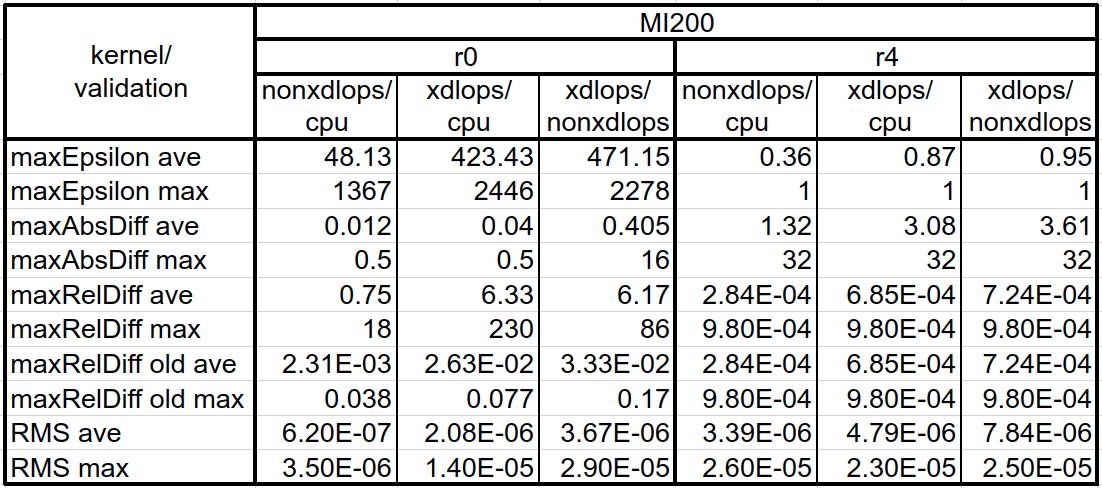
\includegraphics[width=3.8in]{validation_method}}; 

    %% table name
    \node [below right, align=left] at ($(tab TL)+(0, -4.5)$)
    { r0 [-1, 1] vs. r4 [1, 5]};
  \end{tikzpicture}

  \vskip-.5em
  \begin{itemize}
    \uncover<2->
    {\item cpu: sequential implementation of the convolution operation}
    \uncover<3->
    {\item non-xdlops: convert convolution to gemm and compute gemm without \texttt{mfma}}
    \uncover<4->
    {\item xdlops: convert convolution to gemm and compute gemm with \texttt{mfma}}
  \end{itemize}

  \begin{tikzpicture}[overlay, remember picture]
    \coordinate (orig) at (10, 7);
    
    \draw [fill=cyan] (orig) circle (2pt);
    \coordinate (CPU) at ($(orig)+(1, -3.5)$);
    \coordinate (XDLOPS) at ($(orig)+(4.5, -5)$);
    \coordinate (NONXDLOPS) at ($(orig)+(1, -1)$);

    \uncover<2->
    { \node [circle, draw=black, fill=blue!50!white] (CPU node) at (CPU) {CPU};}
    \uncover<3->
    { \node [circle, draw=black, fill=brown!50!white, align=center] (NONXDLOPS node) at (NONXDLOPS) {non-\\xdlops};}
    \uncover<4->
    { \node [circle, draw=black, fill=red!50!white] (XDLOPS node) at (XDLOPS) {xdlops};}
    \uncover<5->
    { \draw (CPU node) -- (XDLOPS node) node [pos=.5, sloped, above] {medium};
      \draw (NONXDLOPS node) -- (CPU node) node [pos=.5, sloped, above] {small};
      \draw (NONXDLOPS node) -- (XDLOPS node) node [pos=.5, sloped, above] {large};}
  \end{tikzpicture}
  
\end{frame}


\begin{frame}
  \frametitle{Exploration of a ``Better" Validation Function}
  
  \begin{columns}
    \column{0.45\linewidth}
    
    \begin{tikzpicture}[overlay, remember picture]
      \coordinate (tab TL) at (0, .5);
      
      \draw [fill=cyan] (tab TL) circle (2pt);

      \node [below right, inner sep=0] at (tab TL){
        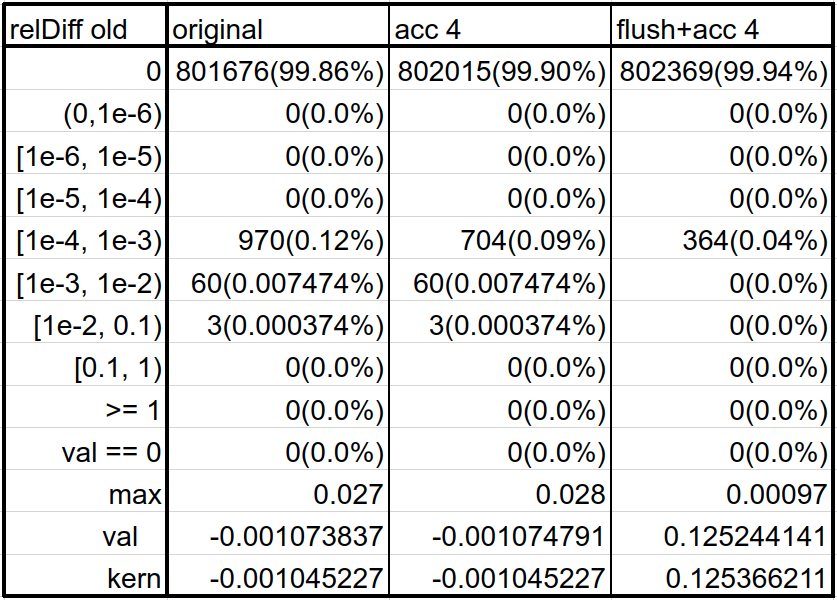
\includegraphics[width=2.8in]{better_validation}}; 

      %% table name
      \node [above right, align=left, scale=.7] at ($(tab TL)+(0,0)$)
      { MI200 xdlops/cpu\\
        \texttt{auto\_e2e/padding\_kernel\_gemmK.mlir [CHECK\_RESNET50\_F16\_CONFIG1]}};
      %% blocker
      \uncover<1>
      { \draw [fill=white, draw=white] ($(tab TL)+(3.33, 0)$) rectangle ++(3.8, -5.2);}
      \uncover<2>
      { \draw [fill=white, draw=white] ($(tab TL)+(5.22, 0)$) rectangle ++(1.9, -5.2);}
      %% Exceptions
      \uncover<2>
      { \draw [blue, thick] ($(tab TL)+(0.03, -1.9)$) rectangle ++(5.22, -.3);}
      \uncover<3->
      { \draw [blue, thick] ($(tab TL)+(0.03, -1.9)$) rectangle ++(7, -.3);
        \draw [red, thick] ($(tab TL)+(0.03, -2.3)$) rectangle ++(7, -.6);
        \draw [brown, thick] ($(tab TL)+(0.03, -4.05)$) rectangle ++(7, -.3);}
      
    \end{tikzpicture}
    
    \column{0.5\linewidth}

    Push CPU to emulate the behavior of the xdlops pipeline
    \begin{itemize}
      \uncover<2->
      {\item \texttt{acc 4}: the \texttt{mfma} instructions are performed by the \texttt{DOT4\_F32\_F16} unit, which performs a fused multiply and add of 4 pairs of fp16 numbers\\
        $\Rightarrow$ truncate the sum of every 4 multiplications from fp64 to fp32\\
        $\Rightarrow$ slightly improves the results}
      \uncover<3->
      {\item \texttt{flush}: flush small numbers ($<2^{-14}$) to zero $\Rightarrow$ greatly improves the results}
    \end{itemize}
  \end{columns}
\end{frame}

\subsection{Summary}
\begin{frame}
  \frametitle{Summary}

  Causes of numerical errors for fp16 tests:
  \begin{enumerate}
  \item Subnormal numbers flushed to zero
  \item Computation order difference due to partition of gemm onto the grid
  \item Truncation behavior difference during accumulation of intermediate results
  \end{enumerate}

  \uncover<2->
  { Element wise vs. RMS
    \begin{itemize}
    \item Element wise metrics are more sensitive to numerical errors\\
      $\Rightarrow$ not suitable for small inputs
    \item RMS is more sensitive to the magnitude of the elements\\
      $\Rightarrow$ not suitable for large inputs
    \end{itemize}}
\end{frame}

\section{Proposals}
\begin{frame}
  \frametitle{Upcoming Testing Framework}
  \begin{enumerate}
  \item Combine RMS and element wise metrics together (MLIR\#620)
    \begin{itemize}
    \item For random inputs with [-1, 1], use RMS
    \item For random inputs with [-3, -1] and [1, 3], use maxRelDiff
    \end{itemize}
  \item Let each test decide how to verify the results (MLIR\#621)
    \begin{itemize}
    \item choose the range of random numbers
    \item choose which metric to use
    \item choose the tolerance for each metric
      \begin{itemize}
      \item RMS: $3\times10^{-5}$
      \item maxRelDiff: $1\times10^{-3}$
      \end{itemize}
    \end{itemize}
  \end{enumerate}
\end{frame}

\end{document}